\chapter{Реализация}
\label{cha:impl}

\section{Разработка}
Разработку модуля необходимо начать с интеграции фреймворка Open SAML 3 с OSGI средой, затем будет рассмотрена разработка модулей авторизации и работы с SAML сообщениями.

\subsection{Интеграция Open SAML 3 со средой OSGI}
Как было выявлено в процессе выбора фреймворка, Open SAML 3 выполняет первоначальную инициализацию, загружая необходимые ресурсы и классы используя загрузчик классов не знающий о существование среды OSGI. Стандартный процесс инициализации фреймворка предполагает вызов метода initialize() сервиса org.opensaml.core.config.InitializationService. Данный сервис загружает все объекты которые необходимы для работы и регистрирует их в Java среде использую Java Services API с помощью сервиса org.opensaml.core.config.ConfigurationService. Для использования фреймворка в OSGI среде необходимо переопределить инициализацию фреймворка и поведение вышеописанных сервисов.

Для решения данной задачи было разработано три класса выполняющие первоначальную инициализацию фреймворка:
\begin{enumerate}
\item Activator - класс в котором заданы действия выполняющиеся при запуске модуля. В данном приложение метод активации извлекает загрузчик классов этого модуля и передает его в класс инициализации Open SAML 3, после чего вызывается метод SamlInitializationSupport.initialize(), листинг \ref{lst:activator}.
\item InitializationXMLConfigurator - класс наследует XMLConfigurator и подменяет загрузчик классов в методе createClassInstance(), листинг \ref{lst:xmlConfigurator}.
\item SamlInitializationSupport - основной класс инициализации, хранит все конфигурации и загрузчик классов модуля, листинг \ref{lst:samlInitialization}. Содержит следующие ключевые методы:
\begin{enumerate}
\item initializeXMLTooling - инициализирует все XML сервисы, перечисленные в списке конфигураций: configs[], использует переопределённый InitializationXMLConfigurator.
\item initializeAlgorithmRegistry -инициализирует алгоритмы используя загрузчик классов модуля.
\item initializeParserPool - инициализирует XML парсер.
\end{enumerate}
\end{enumerate}

\begin{longlisting}
\inputminted[linenos,frame=single]{java}{inc/src/Activator}
\caption{Метод активации модуля} 
\label{lst:activator}
\end{longlisting}

\begin{longlisting}
\inputminted[linenos,frame=single]{java}{inc/src/InitializationXMLConfigurator}
\caption{Класс инициализации XML конфигураций} 
\label{lst:xmlConfigurator}
\end{longlisting}

Данные классы выполняют инициализацию фреймворка Open SAML 3 во время активации модуля. Дальнейшая работа с фреймворком не требует специальных настроек и может выполняться как в классическом Java приложение.

\subsection{Подмодуль authentication}
Данный пакет предназначен для обработки запросов поступающих к сервису и является входной точкой приложения, диаграмма классов пакета представлена в приложение А рис.~\ref{fig:authenticationModule}. Пакет содержит следующие подпакеты и классы:
\begin{enumerate}
\item security.encryption
\item servlets
\item utils
\item Constatns
\item User
\item UserCookie
\end{enumerate}

\paragraph{Пакет security.encryption} содержит классы DesEncryptor и DesDecryptor  выполняющие шифрование и дешифрование значения куки с использованием алгоритма RSA/ECB/PKCS1Padding и стандартного Java класса javax.crypto.Cipher листинг \ref{lst:cipher}. Классы имеют методы decrypt() и encrypt() принимающие в качестве параметров строку которую необходимо зашифровать и ID поставщика сервиса. Ключ для шифрования извлекается из Java хранилища ключей, имя ключа извлекается из конфигурации модуля относящейся к переданному поставщику сервиса.

\begin{listing}[H]
\inputminted[linenos,frame=single]{java}{inc/src/cipher}
\caption{Код получения шифра} 
\label{lst:cipher}
\end{listing}

\paragraph{Пакет servlets} содержит сервлеты которые обрабатывают пользовательские запросы:
\begin{enumerate}
\item LoginServlet - Данный сервлет обрабатывает запросы на авторизацию либо ответы от поставщика учетных записей и имеет два сценария срабатывания:
\begin{enumerate}
\item Если поступил запрос на авторизацию от пользователя, то извлекается ID поставщика сервиса из селектора запроса с помощью которого будет получена конфигурация данного поставщика, затем составляется сообщение для поставщика учетных записей и выполняется его отправка.
\item Если в параметрах запроса обнаружен SAML ответ на авторизацию, то будет вызван обработчик AuthenticationResponseHandler.
\end{enumerate}
\item LogoutServlet -  Данный сервлет обрабатывает запросы на выход из системы либо ответы от поставщика учетных записей и имеет три сценария срабатывания:
\begin{enumerate}
\item Если в параметрах запроса обнаружен SAML ответ на запрос выхода из системы, то будет вызван обработчик LogoutResponseHandler. 
\item Если в параметрах запроса обнаружен SAML запрос на выход из системы, что означает запрос на выход из системы со стороны поставщика учетных записей, то будет вызван обработчик LogoutRequestHandler. 
\item Если поступил запрос на выход из системы от пользователя, получается конфигурация поставщика сервиса по аналогии с запросом авторизации, затем составляется и отправляется сообщение для поставщика учетных записей.
\end{enumerate}
\item UserInfo - Сервлет используемый для тестирования и влидации. Отображает информацию которая хранится о пользователи в куки.
\end{enumerate}

Данный пакет также содержит следующие обработчики запросов:
\begin{enumerate}
\item AuthenticationResponseHandler - обрабатывает и валидирует SAML ответы от поставщика учетных записей с помощью класса SamlAuthnResponseValidator. Если ответ прошел валидацию создается пользователь из полученных параметров SAML Assertion и сохраняются куки пользователя, пользователь перенаправляется на страницу для авторизованных пользователей либо на запрашиваемый ресурс.
\item LogoutRequestHandler - обрабатывает SAML запрос на выход из системы полученный от поставщика учетных записей. Удаляет куки пользователя, формирует и отправляет SAML сообщение для поставщика учетных записей о выполненной операции, после чего переправляет пользователя на страницу для не авторизованных пользователей.
\item LogoutResponseHandler - обрабатывает SAML ответ подтверждающий выход из системы полученный от поставщика учетных записей. Удаляет куки пользователя и переправляет его на страницу для не авторизованных пользователей.
\end{enumerate}

\paragraph{Пакет utils} содержит класс AuthUtils предназначенный для проверки передаваемых параметров на наличие XSS уязвимостей.

\paragraph{Класс Constatns} содержит константы путей по которым доступны сервлеты и значение куки которое должно быть задано при выходе из системы.
\paragraph{Класс User} представляет из себя модель пользователя и содержит все поля которые могут быть переданы поставщиком учетных записей вместе с ответом авторизации.
\paragraph{Класс UserCookie} представляет из себя модель куки пользователя и содержит набор значений которые хранятся в куки для пользователя:
\begin{enumerate}
\item userName - ID авторизованного пользователя.
\item sessionIndex - индекс сессии полученный от поставщика учетных записей.
\item user - объект пользователя полученный от поставщика учетных записей.
\end{enumerate}

\subsection{Подмодуль saml} 
Данный пакет предназначен для работы с SAML сообщениями а также конфигурации модуля, диаграмма классов пакета представлена в приложение А рис.~\ref{fig:samlModule}. Пакет содержит следующие подпакеты и классы:
\begin{enumerate}
\item bundle
\item configuration
\item messages
\item security
\item utils
\item validator
\end{enumerate}

\paragraph{Пакет bundle} содержит единственный класс Activator который был подробно рассмотрен в разделе "Интеграция Open SAML 3 со средой OSGI".
\paragraph{Пакет configuration} содержит сервисы конфигурации которые будут рассмотрены подробно в следующей секции данной главы.
\paragraph{Пакет messages} содержит классы осуществляющие генерацию SAML сообщений которые отправляются поставщику учетных записей и состоит из следующих классов:
\begin{enumerate}
\item BindingType - перечисляемый тип который содержит виды SAML привязки доступные в приложение. В текущей версии поддерживаются только POST и REDIRECT.
\item AbstractSamlMessage - абстрактный класс который содержит общие методы для всех SAML сообщений. Содержит следующие методы для работы с сообщениями:
\begin{enumerate}
\item generateUUID - генерирует ID которое служит идентификатором сообщения.
\item generateSigningParameters - генерирует параметры необходимые для подписи сообщения.
\item appendSigningData - подписывает сообщение в соответствие с типом привязки.
\item signObject - подписывает сообщение с помощью сертификата для типа привязки POST.
\item sendMessageToIDP - собирает сообщение и отправляет его поставщику учетных записей.
\end{enumerate}
\item SAML2AuthnRequestMessage - сообщение авторизации.
\item SAML2LogoutRequestMessage - сообщение выхода из системы.
\item SAML2LogoutResponseMessage - сообщение ответ на запрос выхода из системы со стороны поставщика учетных записей.
\end{enumerate}
\paragraph{Пакет security} содержит класс X509 который осуществляет взаимодействие с Java хранилищем ключей и предоставляет ключи для подписи сообщений или валидации полученных сообщений.
\paragraph{Пакет utils} содержит классы инициализации которые были рассмотрены ранее, а также вспомогательный класс SamlUtils со следующими методами:
\begin{enumerate}
\item getMessage - используется в обработчиках для извлечения SAML сообщения из запроса.
\item getMessageEncoder - используется в SAML сообщениях для задания сообщению кодировщика в соответствие с указанным в конфигурации типом  привязки.
\end{enumerate}
\paragraph{Пакет validator} содержит единственный класс SamlAuthnResponseValidator, который выполняет валидацию SAML ответа от поставщика учетных записей на запрос авторизации. Код валидации представлен на листинге \ref{lst:validation}. В процессе валидации проверяется что структура сигнатуры верна и она подписана сертификатом который принадлежит поставщику учетных записей. Валидатор сигнатуры использует для работы Java Service API и требует отдельного переопределения для использования загрузчика классов модуля, листинг \ref{lst:activator}.

\begin{longlisting}
\inputminted[linenos,frame=single]{java}{inc/src/validatorLoader}
\caption{Код переопределения загрузчика классов валидатора} 
\label{lst:validatorLoader}
\end{longlisting}

\subsection{Конфигурация модуля}
Конфигурация модуля находится в пакете saml и содержит два вида конфигурации:
\begin{enumerate}
\item SamlConfigurationImpl - конфигурация которая содержит все элементы задающие используемый в системе поставщик учетных записей. Имеет следующие параметры:
\begin{enumerate}
\item idp.metadata.uri - URL метаданных IdP из которых извлекаются URL авторизации и выхода из системы.
\item jvm.keystore.location - путь до Java хранилища ключей в системе.
\item jvm.keystore.password - пароль Java хранилища ключей.
\item sp.saml.binding.type - тип SAML привязки, выбираемый параметр который может быть POST или REDIRECT.
\item ids.cookie.expiry - время жизни куки пользователя, если -1 время жизни приравнивается к времени жизни сессии.
\end{enumerate}
\item SamlServiceProviderConfigurationFactory - конфигурация которая задает параметры поставщика сервиса в системе. В системе может использоваться несколько различных поставщиков учетных записей с различными конфигурациями. Имеет следующие параметры:
\begin{enumerate}
\item sp.acs.uri - URL для обработки ответов от IdP и обработки утверждений.
\item sp.name - имя поставщика сервиса.
\item sp.id - идентификатор поставщика сервиса, используется для доступа к данной конфигурации.
\item x509.certificate.alias - имя сертификата который используется для подписи сообщений и валидации ответов от IdP.
\item x509.certificate.password - пароль от сертификата.
\item wcms.ids.cookie.name - имя под которым сохраняются куки пользователя.
\item wcms.ids.redirect.landingPage.url - URL на который переправляется пользователь после успешной авторизации.
\item wcms.ids.error.redirect.url - URL ошибок на который переправляется пользователь при возникновение ошибок в процессе авторизации.
\item wcms.ids.redirect.pattern - проверяет что URL перенаправления валдиный. 
\item cookie.additional.attributes - дополнительные параметры полученные от IdP.
\end{enumerate}
\item IdsConfigurationImpl - вспомогательная конфигурация, которая задает параметры позволяющие пользователю проходить авторизацию на стороне сайта или портала без перехода на сайт IdP. Имеет следующие параметры:
\begin{enumerate}
\item ids.host.name - адрес сервиса.
\item ids.port.number - порт сервиса.
\item ids.logon.ui.script - путь до скрипта пользовательского интерфейса.
\item ids.user.profile.script - путь до скрипта модального окна IdP.
\end{enumerate}
\end{enumerate}

\section{Тестирование}

Тестирование проходило в 2 этапа, локально и на тестовом сервере заказчика.
Для локального тестирования были развернуты – три AEM лэндскейпа.
\begin{itemize}
\item Режимы работы: author, crx3, crx3tar, nosamplecontent.
\end{itemize}

\subsection{Тестирование сценария входа}
Для тестирование сценария входа использовался два ресурса где выполнялся вход с настроенной конфигурацией используемого в компании поставщика учетных записей.
\begin{itemize}
\item post binding
\item redirect binding
\end{itemize}

Ожидаемый результат проверки: "Пользователь успешно залогинен". 
Полученный результат: "Пользователь успешно залогинен".

\subsection{Тестирование сценария выхода}
Для тестирования сценариев выхода было использовано три портала использующих разработанный модуль.
\begin{itemize}
\item пользователь успешно залогинен на одном портале и нажимает кнопку разлогин.
\item пользователь залогинен на 2 порталах и нажимает кнопку разлогин на одном из них
\item пользователь успешно залогинен на 3 порталах и нажимает кнопку на разлогин на одном из них.
\end{itemize}

Ожидаемый результат операции: "OK". 
Полученный результат: "OK".

%\subsection{Блок-схема всякой ерунды}
%
%\subsubsection*{Кстати о заголовках}
%
%У нас есть и \Code{subsubsection}. Только лучше её не нумеровать.

\section{Конфигурация в системе}

Приложения использующие модуль должны добавить к себе файл с конфигурацией (ссылка на XML файл, пример) либо заполнить конфигурацию в ручном режиме, однако такой подход не рекомендуется.

\paragraph{Конфигурация поставщика сервиса}
Поставщик сервиса содержит следующий набор конфигураций.
\begin{itemize}
\item cookieexpire
\end{itemize}

\begin{figure}[H]
  \centering
  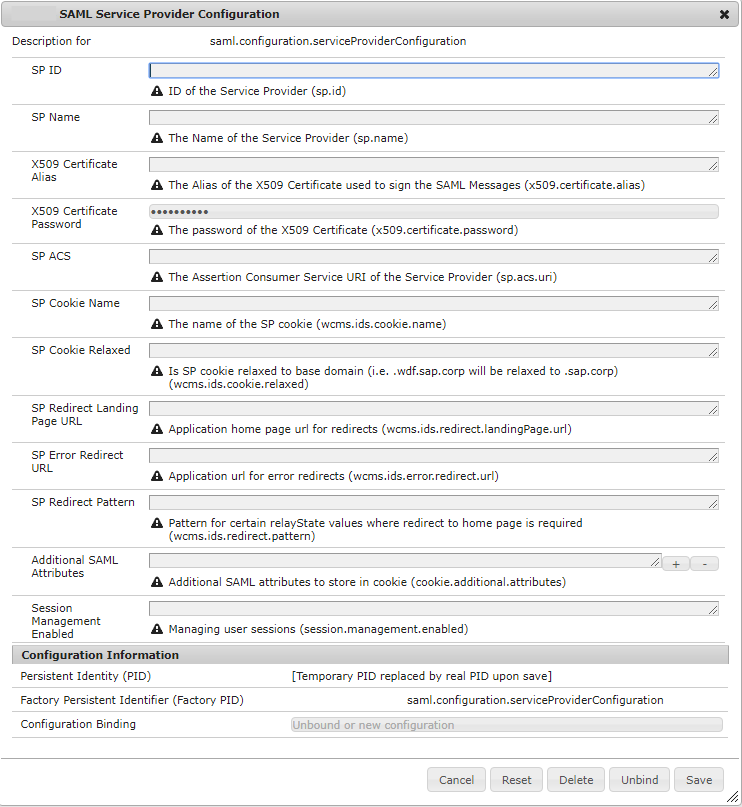
\includegraphics[width=\textwidth]{inc/svg/provider}
  \caption{Конфигурация поставщика сервиса}
  \label{fig:runConfig}
\end{figure}

\begin{listing}[H]
\inputminted[linenos,frame=single]{java}{inc/src/samlProviderConfiguration}
\caption{Код получения шифра} 
\label{lst:samlProviderConfiguration}
\end{listing}

\paragraph{Конфигурация поставщика учетных записей}

\begin{figure}[H]
  \centering
  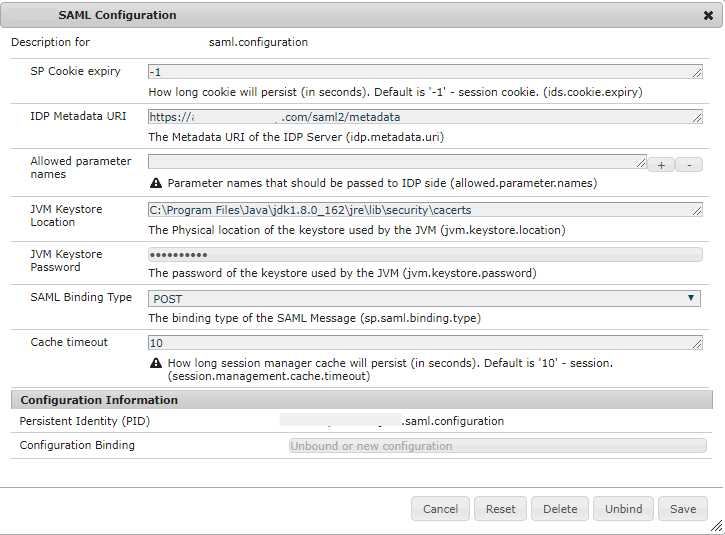
\includegraphics[width=\textwidth]{inc/svg/saml-config}
  \caption{Конфигурация поставщика учетных записей}
  \label{fig:samlConfig}
\end{figure}

\begin{listing}[H]
\inputminted[linenos,frame=single]{java}{inc/src/samlConfiguration}
\caption{Код получения шифра} 
\label{lst:samlConfiguration}
\end{listing}

\paragraph{Конфигурация скрипта}

\begin{figure}[H]
  \centering
  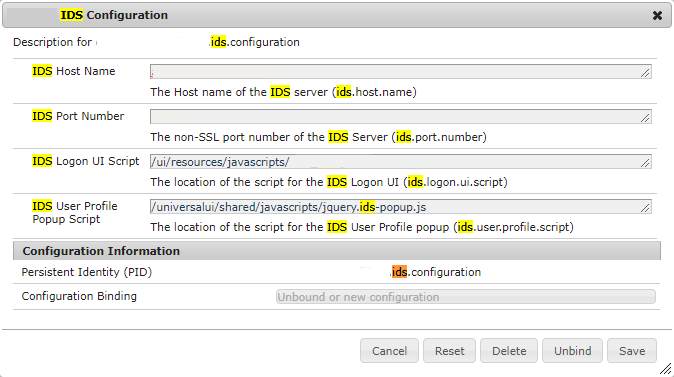
\includegraphics[width=\textwidth]{inc/svg/idsConfig}
  \caption{Конфигурация javascript}
  \label{fig:idsConfig}
\end{figure}

\begin{listing}[H]
\inputminted[linenos,frame=single]{java}{inc/src/idsConfiguration}
\caption{Код получения шифра} 
\label{lst:idsConfiguration}
\end{listing}

%%% Local Variables:
%%% mode: latex
%%% TeX-master: "rpz"
%%% End:

